\section{ 串口调试相关函数 }
\subsection{ 串口初始化函数 }
\begin{figure}[h]
    \centering
    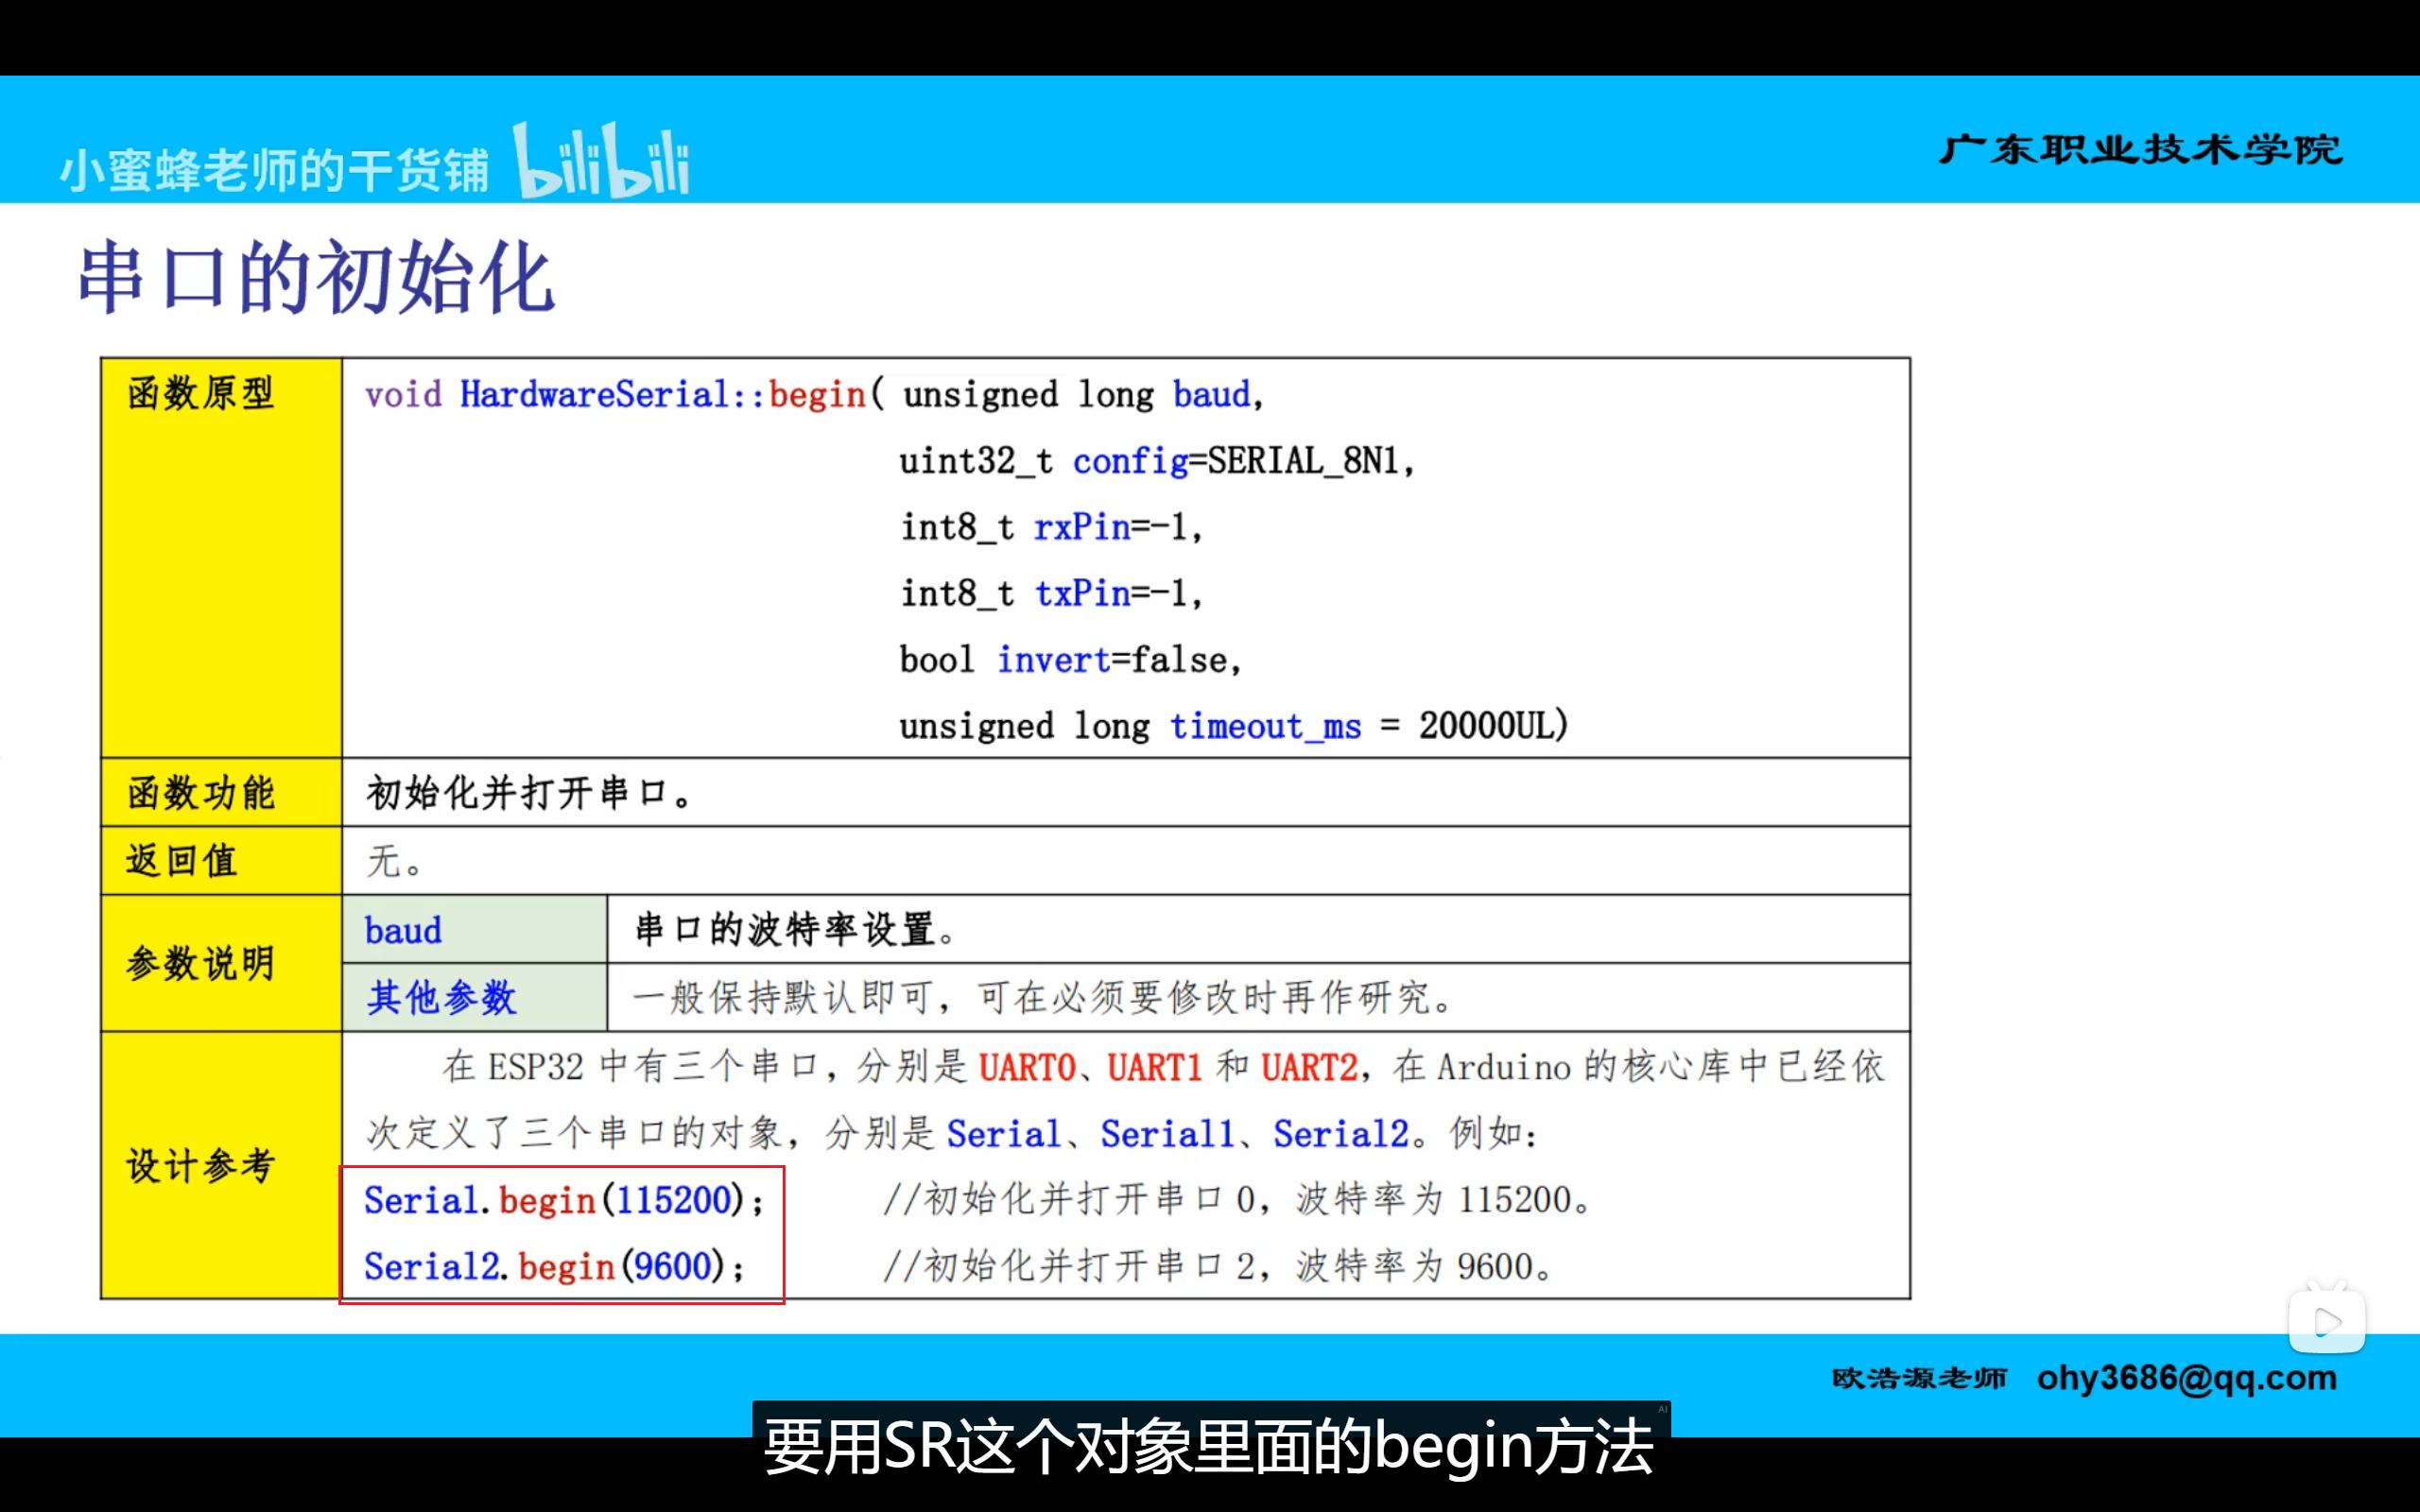
\includegraphics[width=\textwidth]{Figures/Serial.png}
    \caption{Serial}
\end{figure}
函数原型为: \textit{ \textbf{void HardwareSerial::begin} },它有四个参数,第一个参数为要设置的波特率;第二个参数指定串口的数据帧格式，类型为 \textbf{uint32\_t}，默认值为\textbf{ SERIAL\_8N1};
第三第四个参数分别为要重映射的Tx、Rx引脚
\par
在使用时,其实只需要使用\textit{\textbf{Serial.begin,Serial1.begin,Serial.begin}},分别表示\textbf{UART0,UART1,UART2};在设置参数时,大多数情况下只需要设置第一个参数波特率即可
\newpage
\subsection{ 串口打印函数 }
\begin{figure}[h]
    \centering
    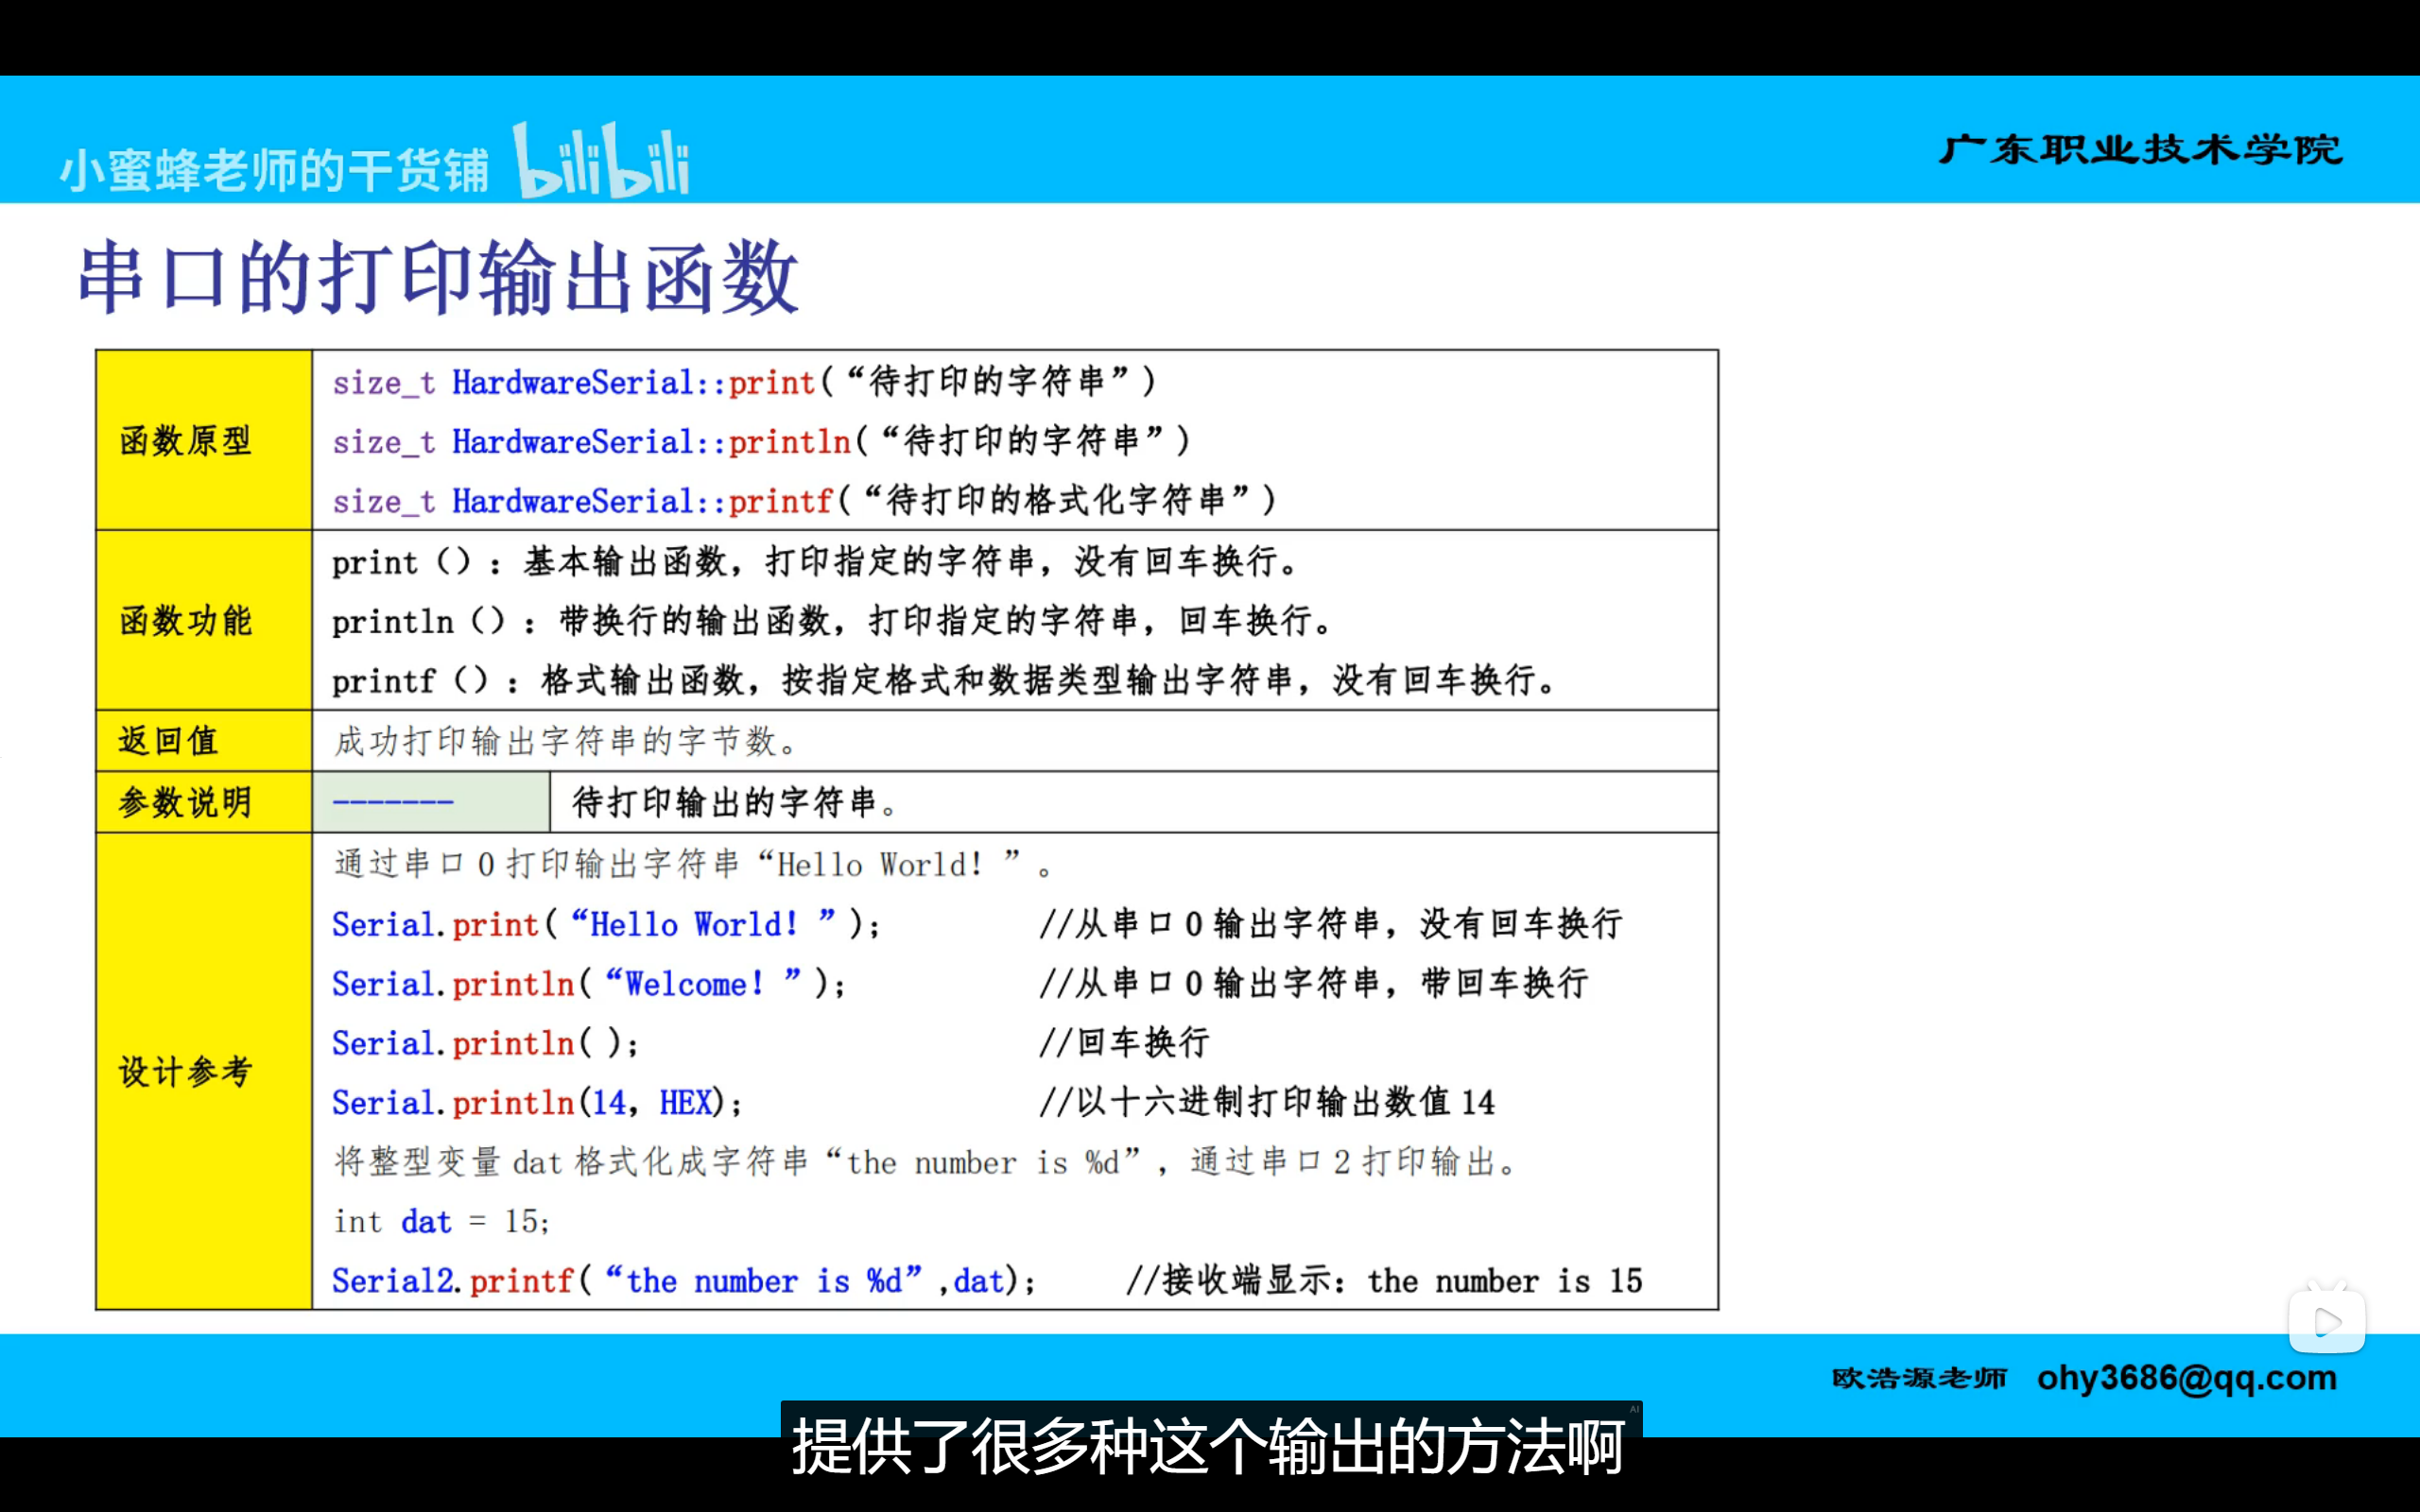
\includegraphics[width=\textwidth]{Figures/Serial_Print.png}
    \caption{Serial打印函数}
\end{figure}
这些函数和上述所说的串口初始化函数用法相似,在实际使用的时候亦是使用\textbf{Serial}(后面添1或者2,不加任何东西表示使用USART0)\textbf{.功能函数名}
\subsection{ 单字符串口写入/读取函数 }
\begin{itemize}
    \item \textit{\textbf{ Serial.write(uint8\_t c) }}:单字符写入
    \item \textit{\textbf{ Serial.read(void)}}:单字符读取
    \item  \textit{\textbf{Serial.available(void)}}:返回该Serial串口缓存区中所有字节的长度
\end{itemize}
\textbf{注意:}
\begin{itemize}
    \item 每个Serial后面都可以加1或2,表示用特定的Serial,不加任何数字表示使用USART0
    \item write、read都是重载函数,即可以往这些函数填入多个参数,根据填入参数数量的不同,函数的功能会发生相应的变化(在下一节中将提到)
\end{itemize}


\newpage
\subsection{ 字符串写入/读取函数(多字符) }
\begin{itemize}
    \item 字符串写入函数(单片机给电脑发送消息):Serial.write(参数一,参数二).参数一为要读取数据的地址(数组名或者指针);参数二为要读取数据的长度.
    \item  字符串读取函数(读取电脑给单片机发送的消息):Serial.read(参数一,参数二).参数一表示要把数据存储到哪个数组(同上),参数二为要读取的长度
\end{itemize}
\par
在读取函数的代码实现中,我们一般先定义一个变量(假设为a),将Serial.available()返回的数据长度赋值给a.这样a就可以作为Serial.read的第二个参数了(表示把缓存区里面的数据全部读取出来). 两个函数具体如下:
\begin{figure}[h]
    \begin{minipage}{0.48\textwidth}
        \centering
        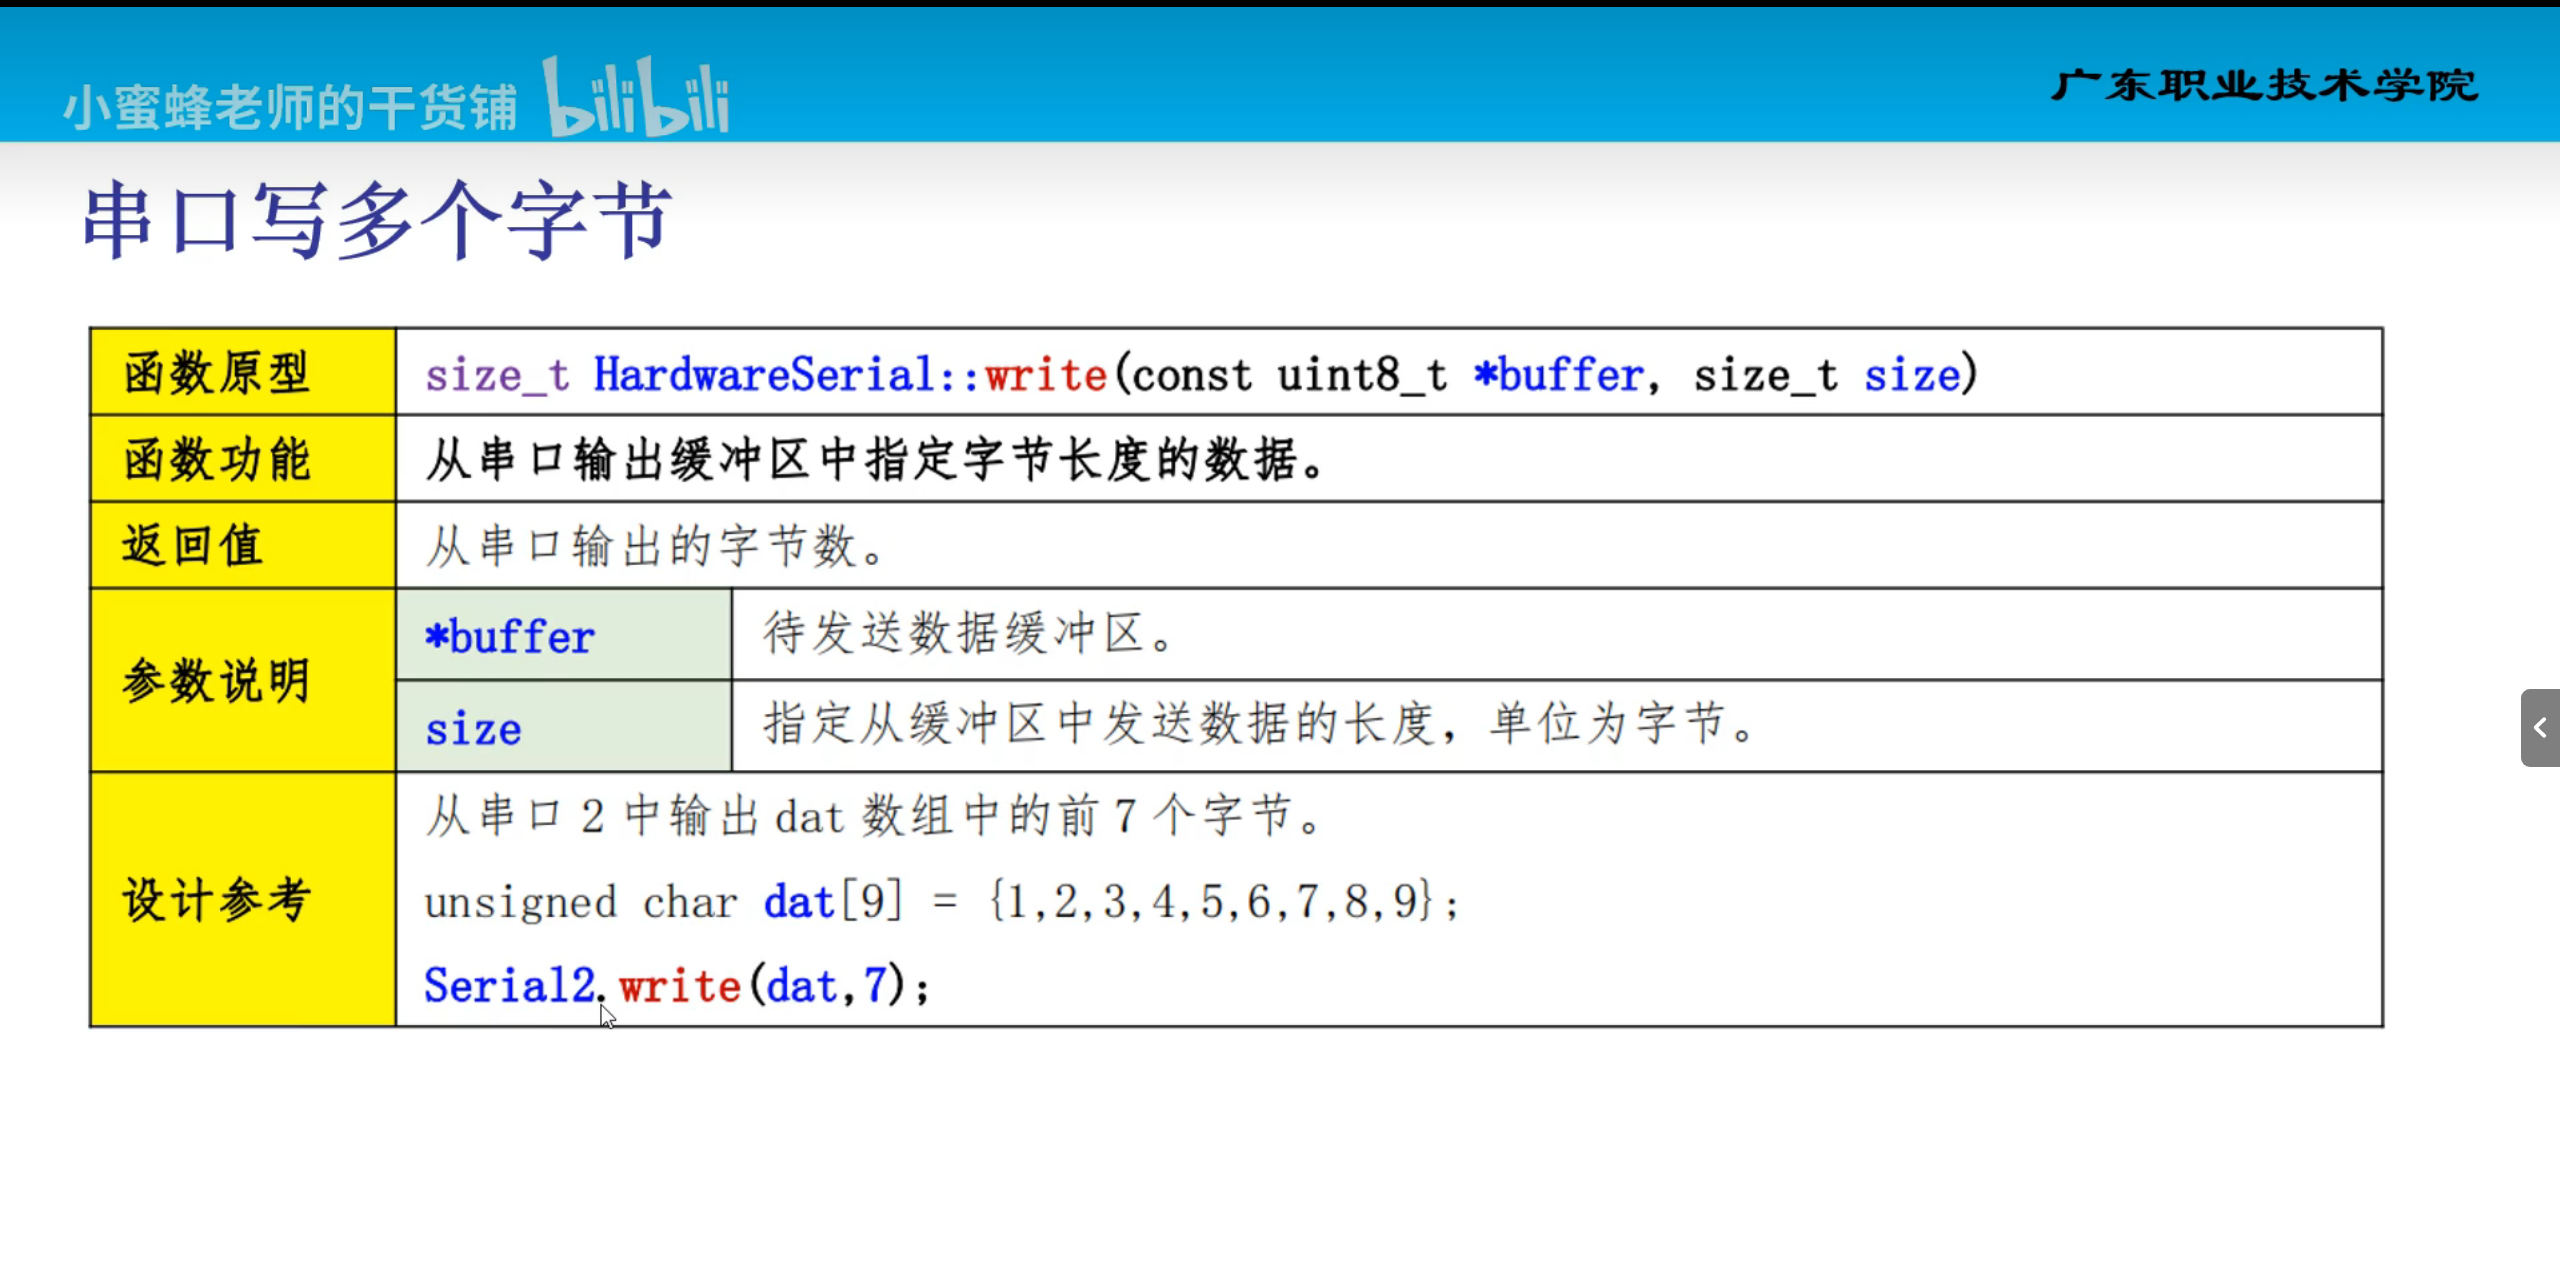
\includegraphics[width = 0.8\textwidth]{Figures/Serial-write.png}
        \caption{Serial.write}
    \end{minipage}
    \begin{minipage}{0.48\textwidth}
        \centering
        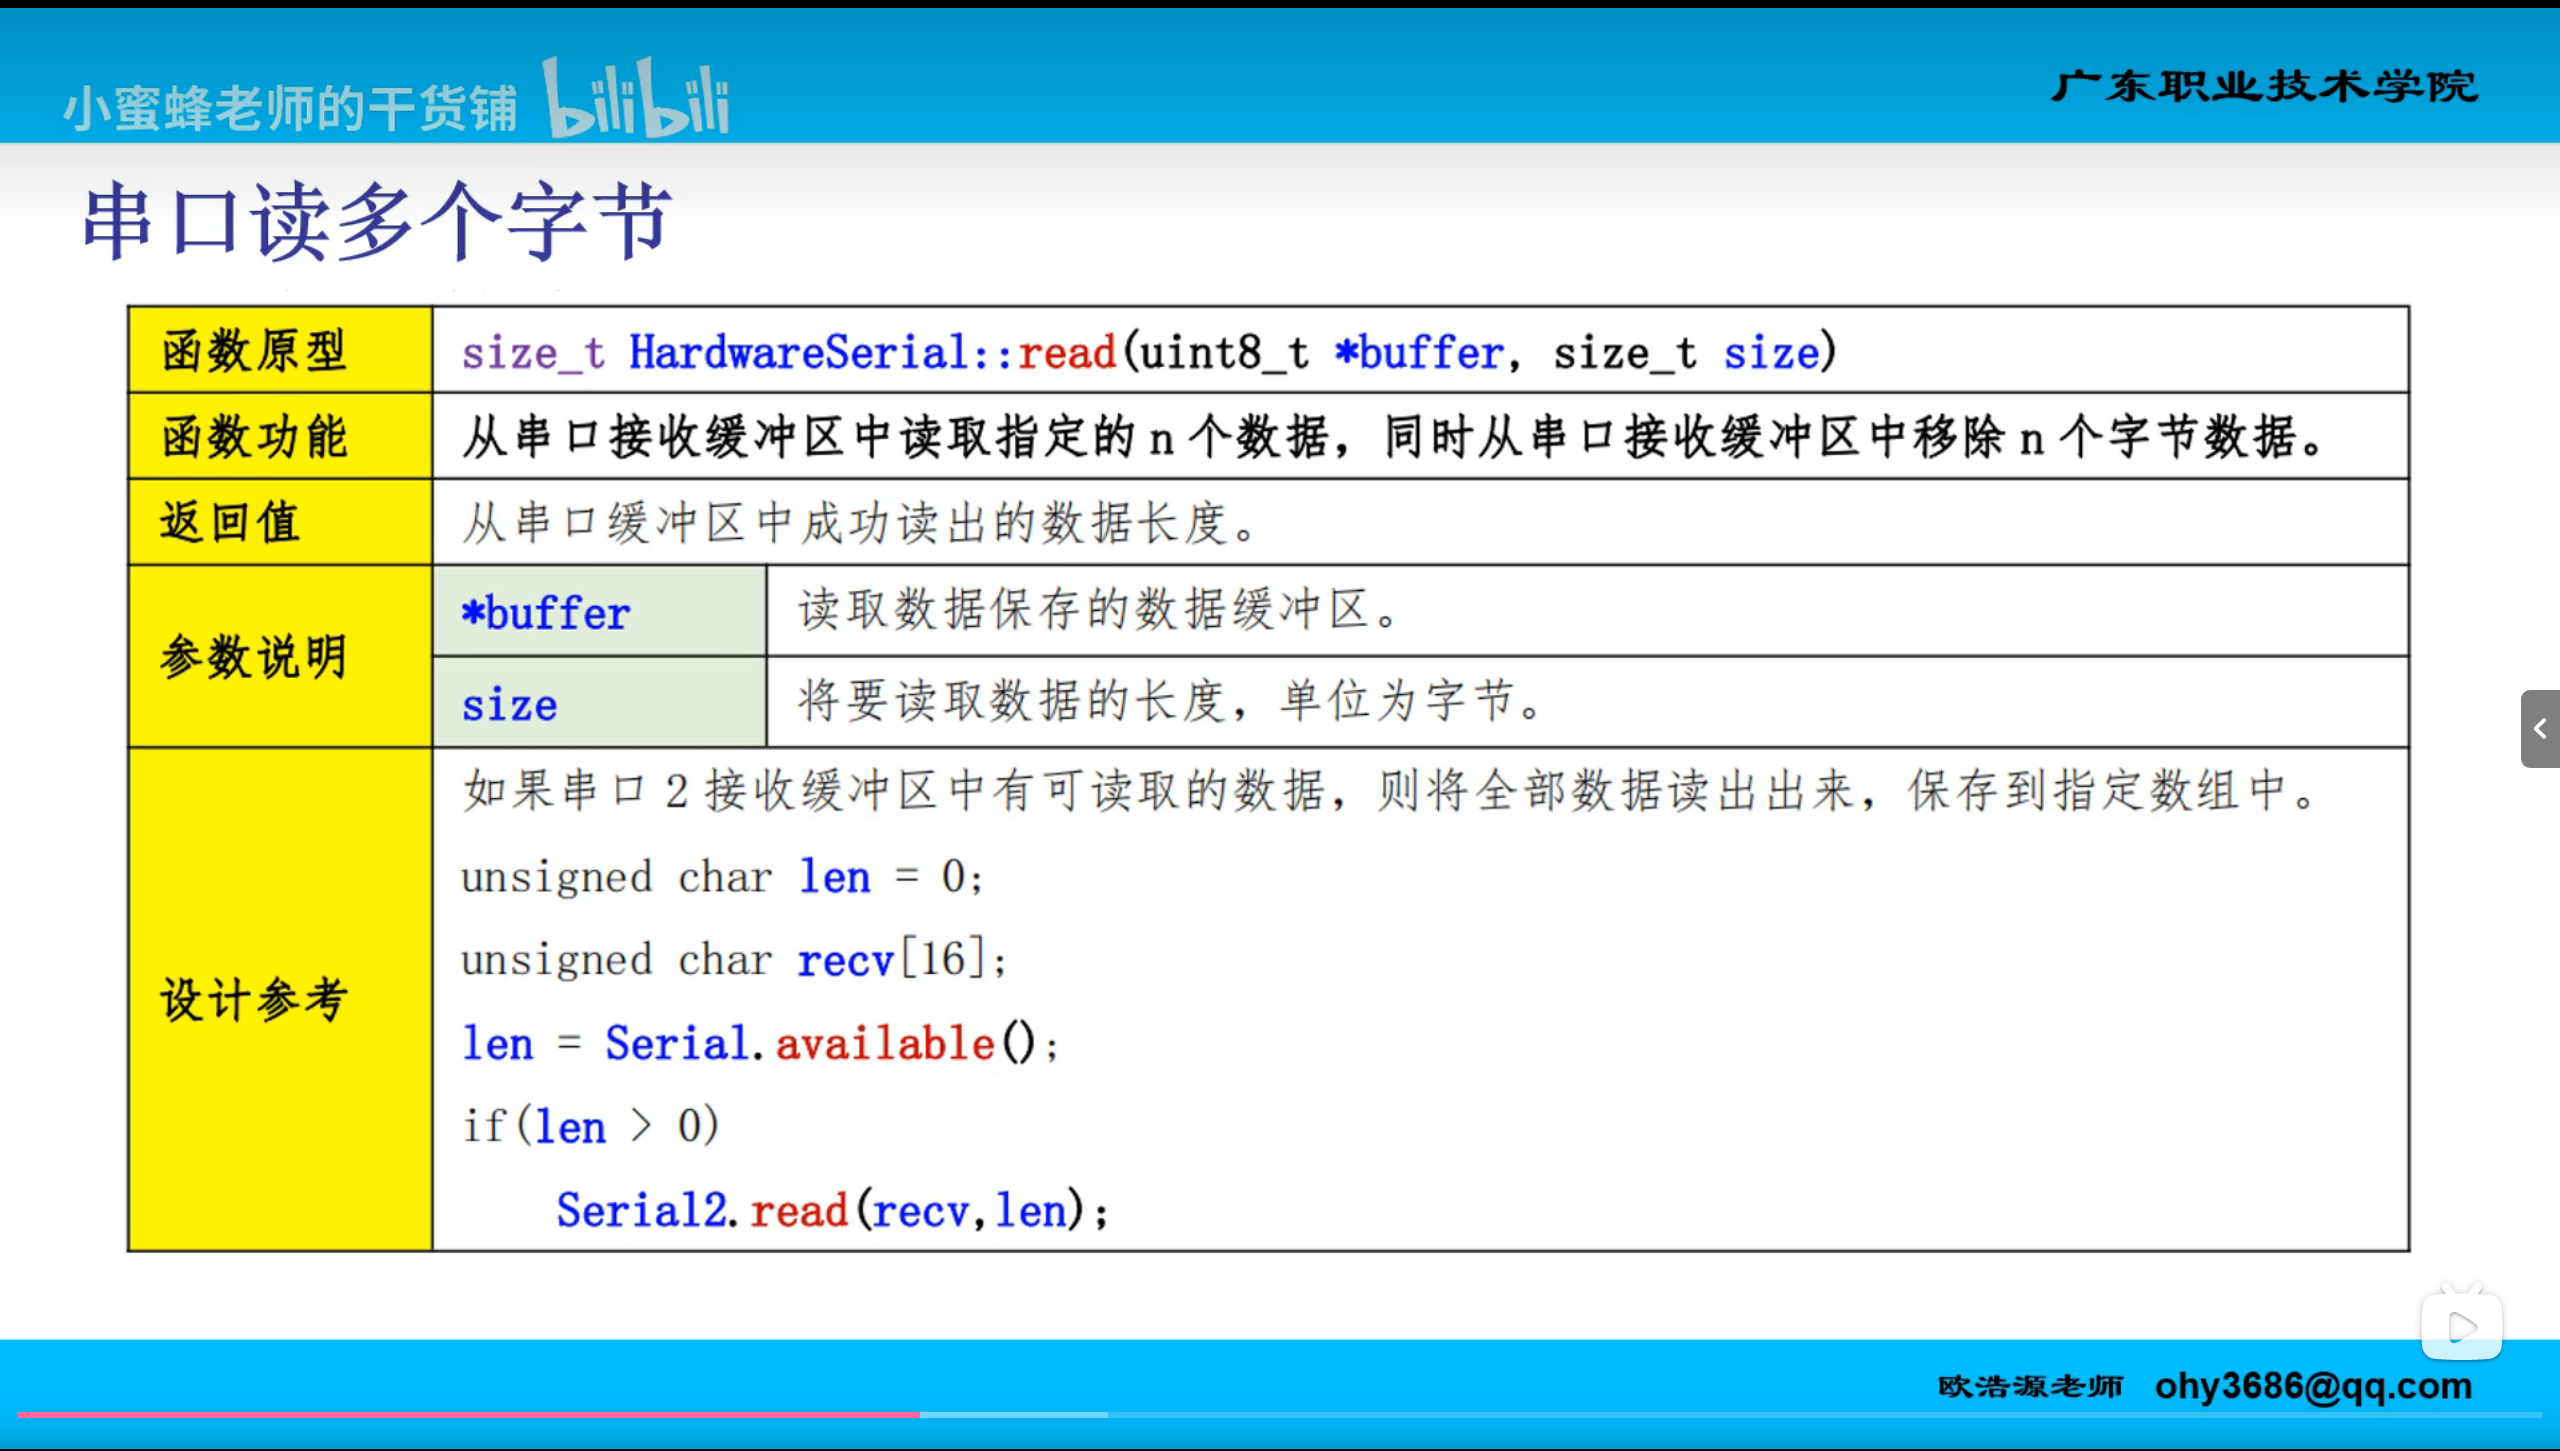
\includegraphics[width = 0.8\textwidth]{Figures/Serial-read.png}
        \caption{Serial.read}
    \end{minipage}
        
    
\end{figure}
\subsection{ 使用串口时注意的事项 }
如果在用USART0进行调试时遇到无法接收任何消息,但是又没有报错的情况,那么可以去platformio.ini文件里面增加这几段代码:
\begin{verbatim}
monitor_speed = 115200
monitor_port = COM7
upload_port = COM7
build_flags =
    -DARDUINO_USB_MODE=1
    -DARDUINO_USB_CDC_ON_BOOT=0
\end{verbatim}
\newpage
如图所示:
\begin{figure}[h]
    \centering
    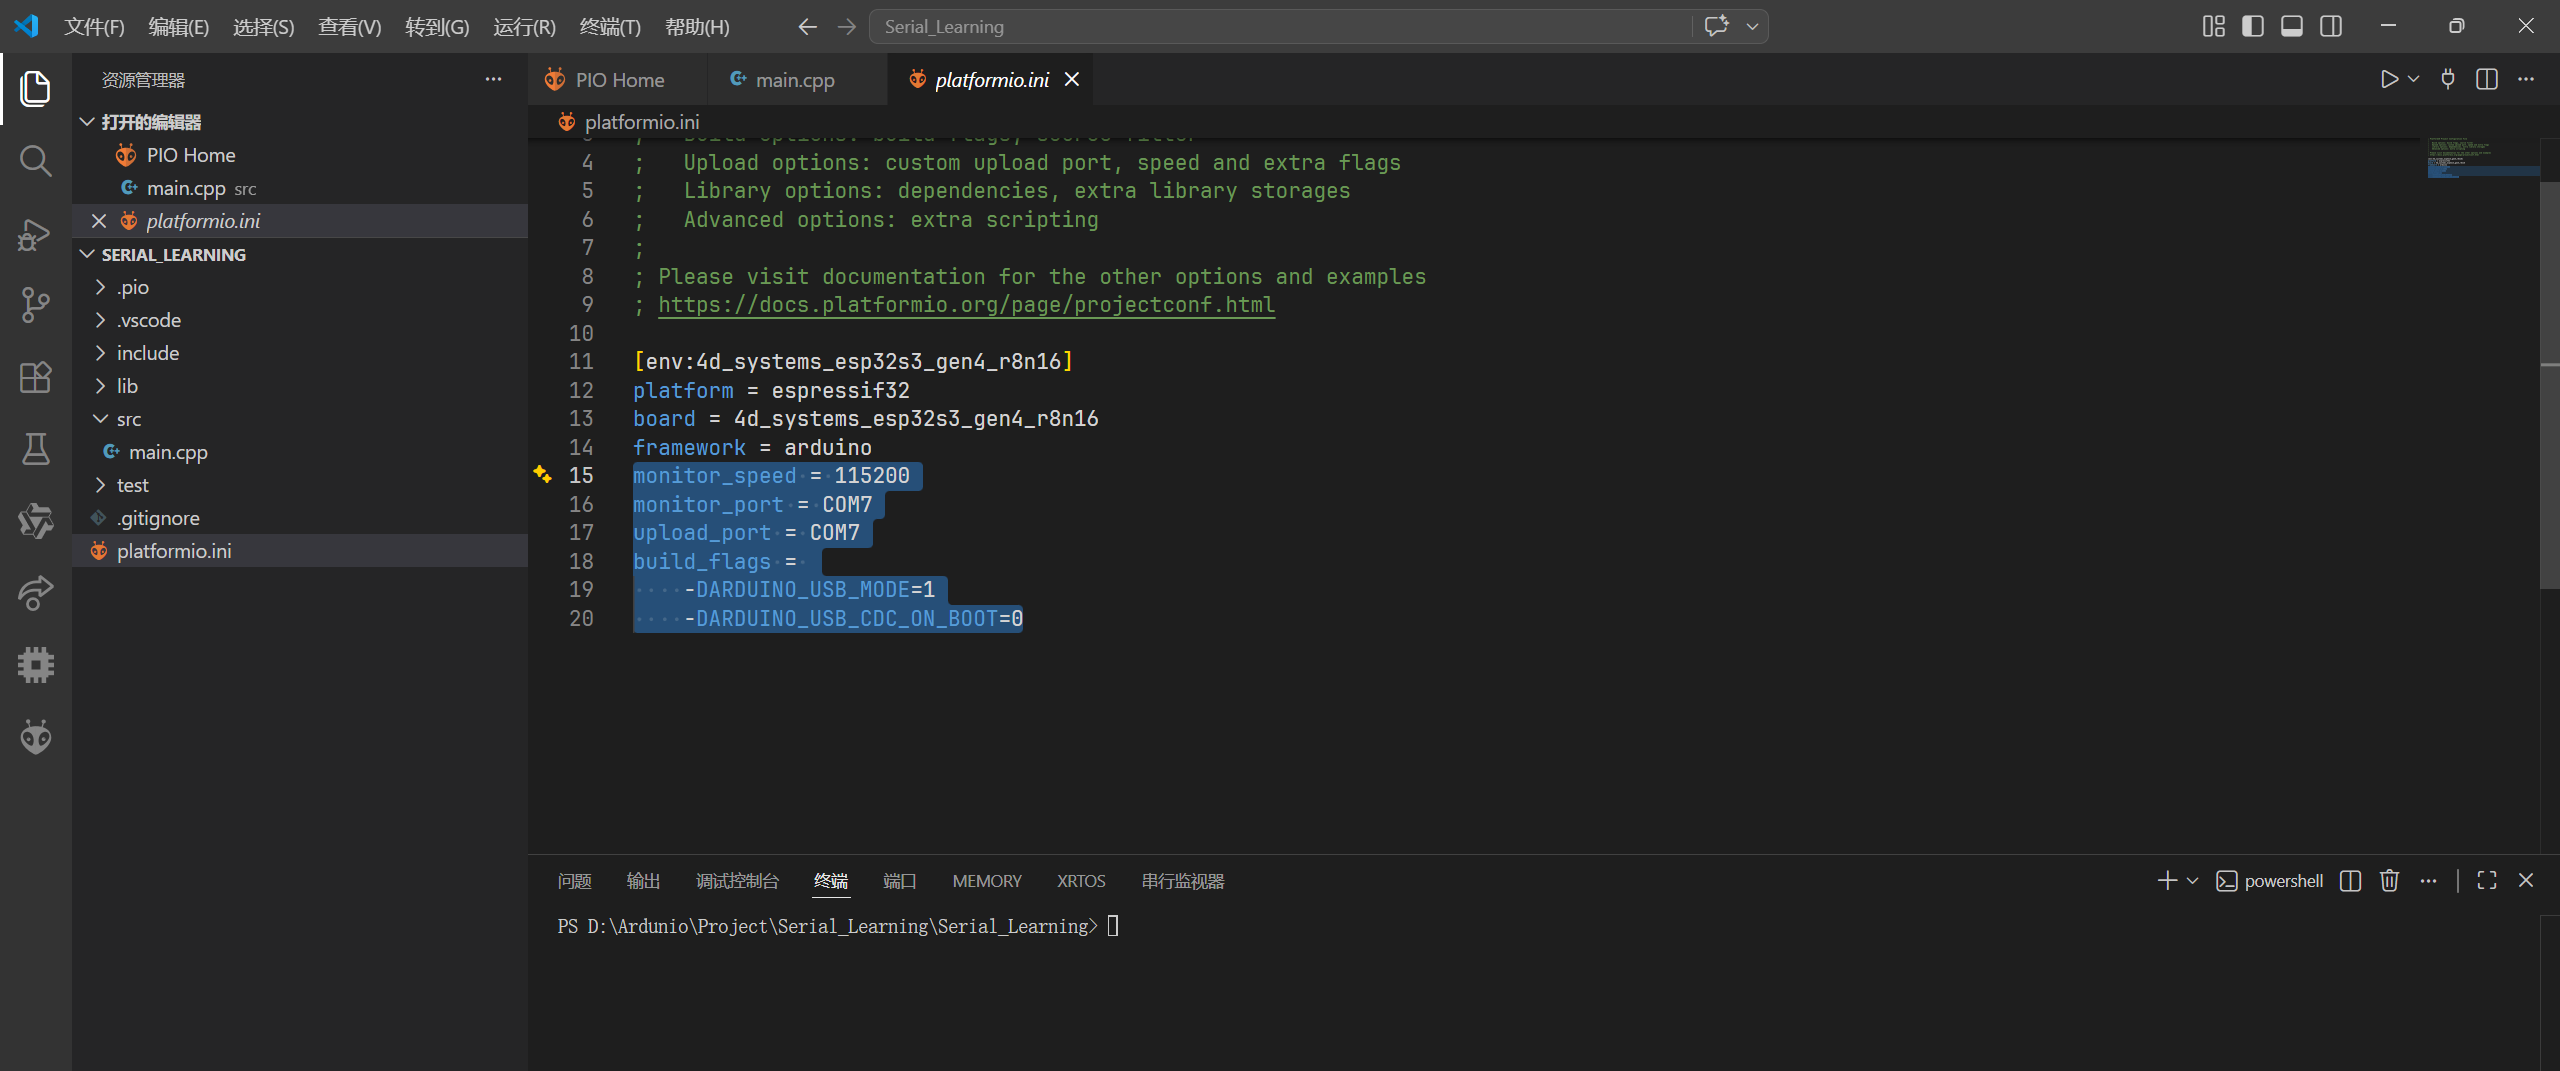
\includegraphics[width=\textwidth]{Figures/System_Build_Structure.png}
    \caption{Caption}
    \label{fig:placeholder}
\end{figure}
\par
这几段代码的作用分别为:
\begin{itemize}
    \item monitor\_speed：设置串口波特率。
    \item monitor\_port / upload\_port：指定使用 COM7，避免自动检测错误。
    \item -DARDUINO\_USB\_MODE=1：禁用原生 USB CDC，串口走 UART0（CH343）。
    \item -DARDUINO\_USB\_CDC\_ON\_BOOT=0：启动时不初始化 USB CDC，确保 Serial 映射到 UART0。
\end{itemize}

\noindent
\par
总结：  
默认情况下，Serial 被映射到原生 USB CDC，而硬件连接的是 CH343（UART 转 USB）。两者不匹配导致无法接收数据。通过上述配置，将 Serial 强制映射到 UART0，从而恢复通信。